\documentclass[11pt,a4paper]{article}
\usepackage[T1]{fontenc}
\usepackage[utf8]{inputenc}
\usepackage{lmodern}
\usepackage{microtype}
\usepackage{geometry}
\usepackage{amsmath,amssymb}
\usepackage{graphicx}
\usepackage{booktabs,tabularx,array}
\usepackage{float}
\usepackage{fancyhdr}
\usepackage{titlesec}
\usepackage[hidelinks]{hyperref}
\usepackage{xurl}
\usepackage{enumitem}
\geometry{left=24mm,right=24mm,top=23mm,bottom=23mm,headheight=15pt,headsep=9mm,footskip=13mm}
\setlength{\parindent}{0pt}
\setlength{\parskip}{5.2pt}
\renewcommand{\arraystretch}{1.16}
\setlength{\tabcolsep}{6pt}
\titleformat{\section}{\large\bfseries}{\thesection}{1em}{}
\titlespacing*{\section}{0pt}{13pt}{5pt}
\titleformat{\subsection}{\normalsize\bfseries}{\thesubsection}{0.75em}{}
\titlespacing*{\subsection}{0pt}{9pt}{4pt}
\pagestyle{fancy}
\fancyhf{}
\fancyhead[L]{\small Introduction to Vehicles and Sensors}
\fancyhead[R]{\small GPS decoding and analysis}
\fancyfoot[C]{\small\thepage}
\renewcommand{\headrulewidth}{0pt}
\renewcommand{\footrulewidth}{0pt}
\setlist[itemize]{leftmargin=*,topsep=2pt,itemsep=2pt,parsep=0pt}
\graphicspath{{GPS_results/}}
\newcommand{\sourcename}[1]{\texttt{#1}}
\begin{document}

\begin{center}
  {\LARGE\bfseries GPS decoding and analysis\par}
  \vspace{4pt}
  {\normalsize Introduction to Vehicles and Sensors\par}
  \vspace{3pt}
  {\normalsize Do Ba Quang Huy\_IFRoS\_OVK57S\par}
\end{center}
\vspace{5pt}

\section{Problem and input data}

Two raw GPS recordings were provided in the NMEA 0183 ASCII format:
\sourcename{nmea-test1-1.txt} and \sourcename{nmea-test2-1.txt}. The objective is to identify which recording was obtained while the receiver was stationary and which while it was moving, describe the positions and movement, estimate horizontal GPS precision, and extract additional information from the NMEA sentences. Both files contain data dated \textbf{4 November 2025 (UTC)}.

\section{Decoding method and calculations}

The analysis was implemented in Python 3 using NumPy and Matplotlib. Each NMEA sentence was first checked using the XOR checksum following the \texttt{\$...*hh} convention. The parser reads \texttt{GGA}, \texttt{RMC}, \texttt{GSA}, \texttt{GSV} and \texttt{VTG}. A position is accepted only if its \texttt{RMC} status is \texttt{A}, the coordinates are available, and the corresponding \texttt{GGA} fix-quality indicator is greater than zero.

NMEA coordinates use degrees and decimal minutes. For a positive north/east value, the conversion to decimal degrees is
\begin{equation}
  \theta_{\mathrm{deg}}=D+\frac{M}{60}.
\end{equation}
For example, \texttt{4728.4485,N} corresponds to $47+28.4485/60=47.47414167^{\circ}$ N, and \texttt{01903.4846,E} corresponds to $19.05807667^{\circ}$ E. South and west coordinates would receive negative signs.

The distance between successive valid geographic positions was calculated with the haversine formula,
\begin{align}
 a &= \sin^2\!\left(\frac{\phi_2-\phi_1}{2}\right)
 + \cos\phi_1\cos\phi_2\sin^2\!\left(\frac{\lambda_2-\lambda_1}{2}\right), \\
 d &= 2R\arcsin(\sqrt{a}), \qquad R=6{,}371{,}000\ \mathrm{m},
\end{align}
where latitude $\phi$ and longitude $\lambda$ are in radians. The reported \texttt{RMC} speed was converted from knots to km/h using $v_{\mathrm{km/h}}=1.852\,v_{\mathrm{knots}}$.

\section{Implementation and execution}

The supplied script, \sourcename{GPS\_analysis.py}, runs from the folder containing the two text files. On a system with Python~3.10 or later, install the dependencies and run:
\begin{quote}
\ttfamily\small
python3 -m pip install -r requirements.txt\\
python3 GPS\_analysis.py nmea-test1-1.txt nmea-test2-1.txt\\
\hspace*{1em}--out-dir GPS\_results
\end{quote}
The program prints decoded statistics in the terminal and saves \texttt{trajectories.png}, \texttt{speeds.png}, \texttt{stationary\_scatter.png}, and two decoded CSV files in \texttt{GPS\_results/}. To save all printed statistics, append \texttt{> GPS\_results\_stats.txt} to the run command. On Windows, \texttt{python} may be used instead of \texttt{python3}. No graphical window is required.

\clearpage
\section{Q1: Stationary and moving recordings}

\begin{table}[H]
\centering
\small
\caption{Comparison of the two recordings using accepted GPS fixes.}
\begin{tabularx}{\textwidth}{@{}Xrr@{}}
\toprule
Measurement & Test 1 & Test 2 \\
\midrule
Valid GPS positions & 219 / 231 & 327 / 327 \\
Valid period (UTC) & 09:06:02--09:09:40 & 09:11:41--09:17:07 \\
Duration with valid fixes & 218 s & 326 s \\
Mean / maximum reported speed & 0.87 / 2.31 km/h & 3.95 / 6.96 km/h \\
Track length from successive points & 80.3 m & 393.8 m \\
Start-to-end displacement & 10.5 m & 24.0 m \\
Satellites used for fix & 3--5 & 6--7 \\
Median HDOP & 2.17 & 1.56 \\
\bottomrule
\end{tabularx}
\end{table}

\begin{figure}[H]
\centering
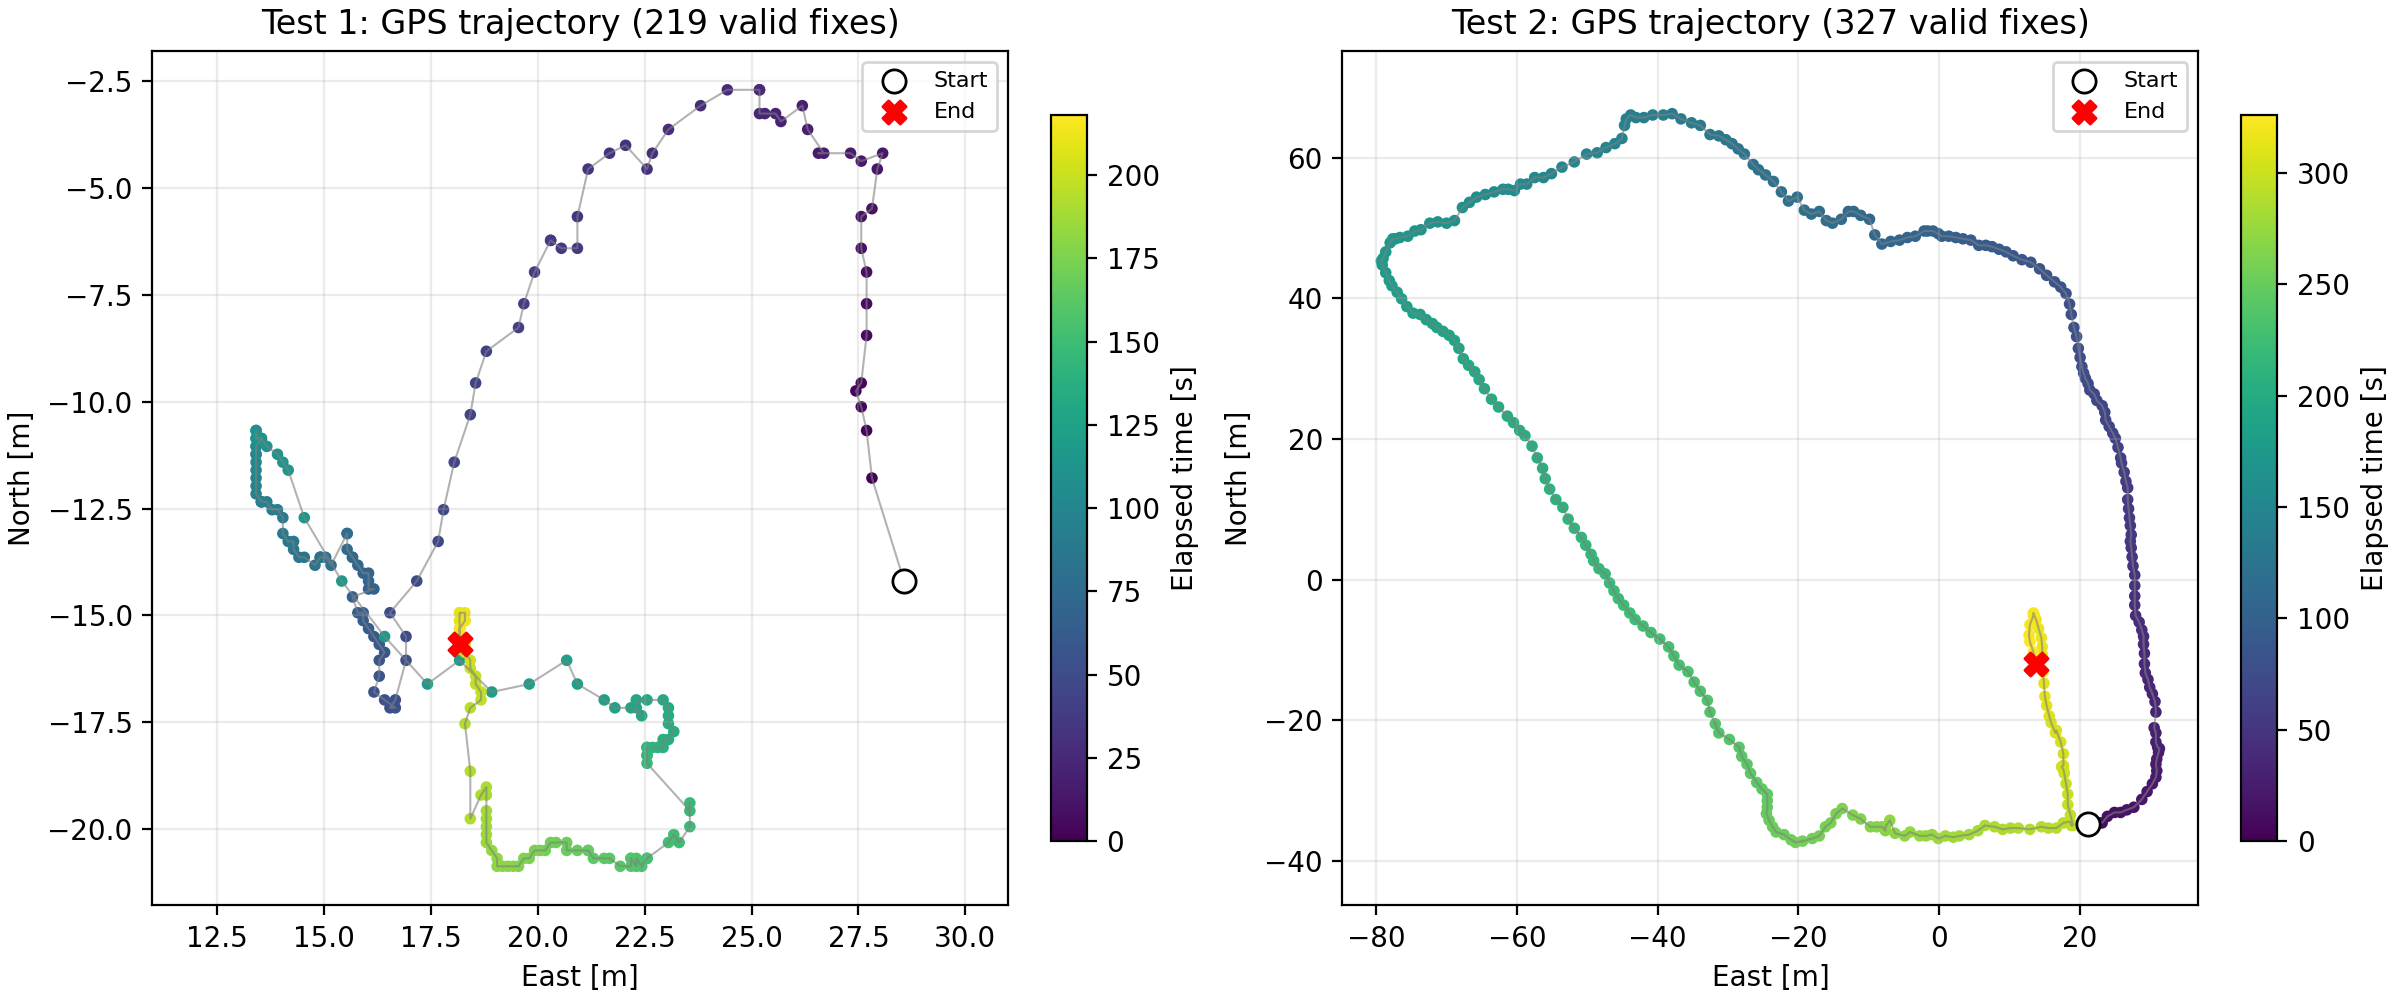
\includegraphics[width=0.92\textwidth]{trajectories.png}
\caption{GPS trajectories in local east/north coordinates. Color indicates elapsed time; a white circle and red cross mark the start and end.}
\end{figure}

\textbf{Test 1 is the stationary recording.} The measured positions remain close to one area; $72.6\%$ of reported speeds are below $1\ \mathrm{km/h}$. GPS scatter and occasional satellite-geometry changes explain its small apparent movement. The mean of its 219 valid positions is approximately $47.47414195^{\circ}$ N, $19.05795521^{\circ}$ E.

\textbf{Test 2 is the moving recording.} Its positions form a much larger curved route with several changes of direction. It starts at $47.47395667^{\circ}$ N, $19.05797833^{\circ}$ E and ends at $47.47416167^{\circ}$ N, $19.05788000^{\circ}$ E. The final position is about 24 m from the start, consistent with a short loop or a return near the starting area.

\clearpage
\begin{figure}[H]
\centering
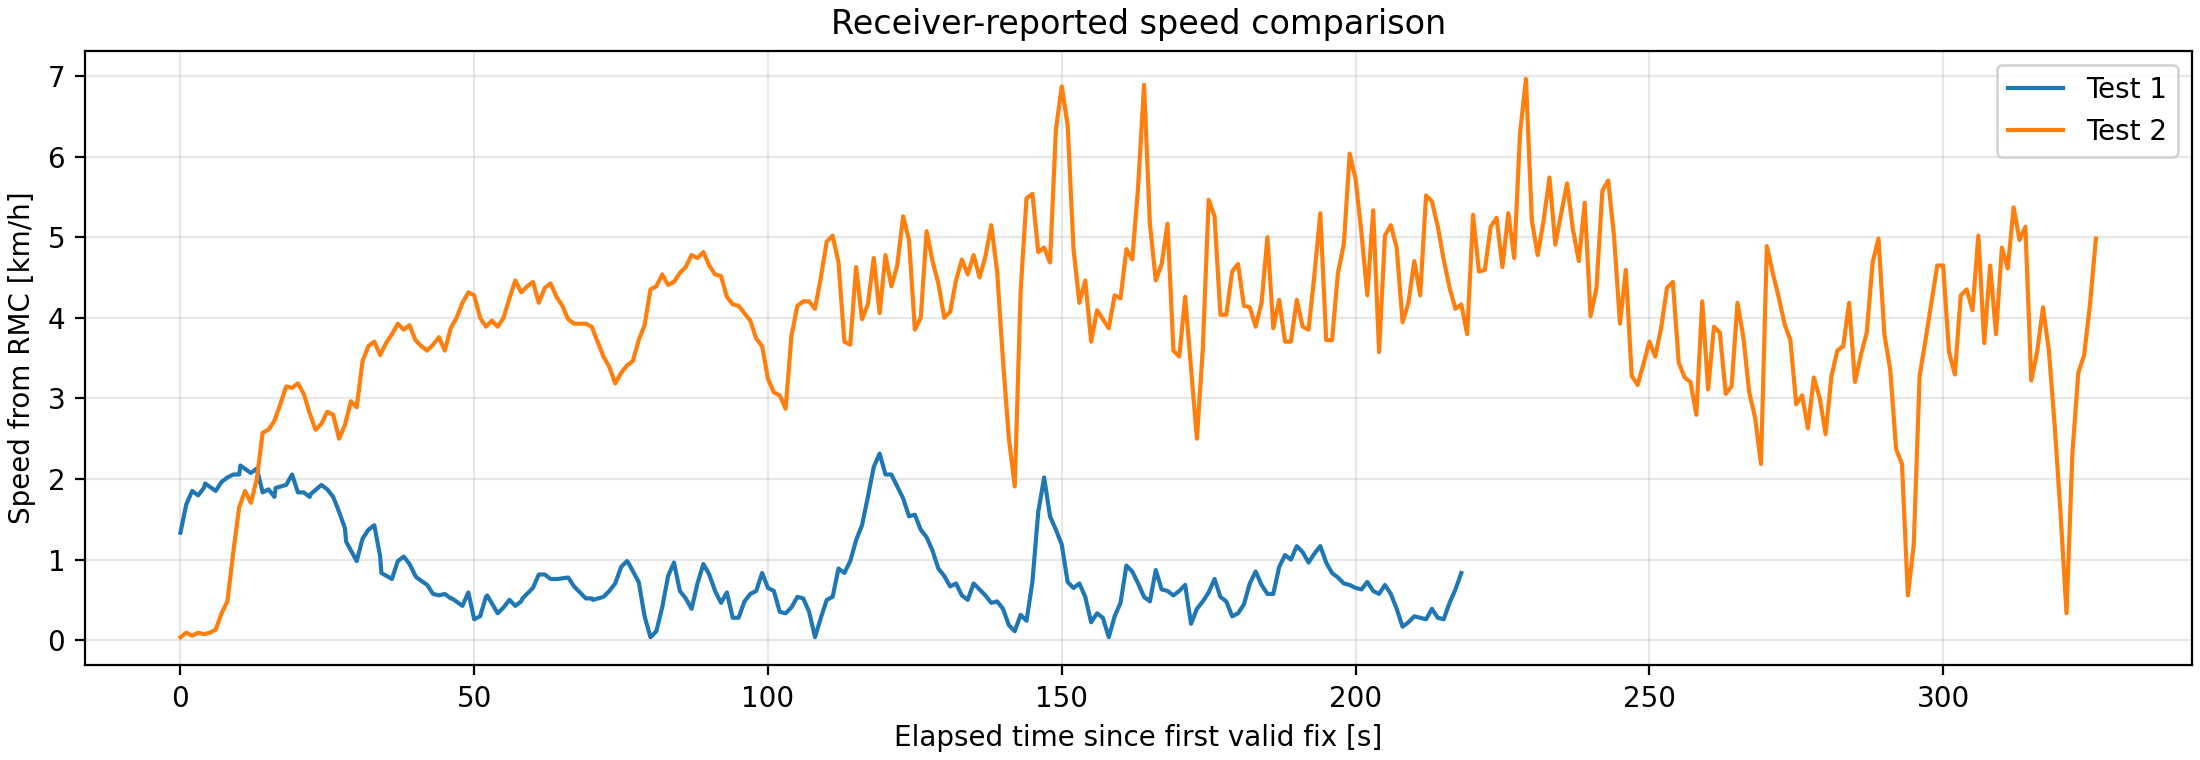
\includegraphics[width=0.91\textwidth]{speeds.png}
\caption{Receiver-reported speed versus elapsed time. The high speed of Test 2 over most of its recording supports the movement classification.}
\end{figure}

Both tracks are located in \textbf{Budapest, Hungary}, in the Buda-side university area near the Danube. The speeds in Test 2 are consistent with \emph{walking}, but a receiver log alone cannot prove the activity or identify the exact streets used. The recorded track lengths are sums of distances between noisy GPS fixes and therefore must not be treated as ground-truth traveled distances. In particular, the 80.3 m cumulative track length in Test 1 is predominantly apparent motion caused by position drift.

\section{Q2: GPS precision and accuracy}

\textbf{Precision} describes the spread of repeated position estimates; \textbf{accuracy} describes their closeness to the true location. As no surveyed reference position is supplied, only internal precision/repeatability can be estimated from the stationary recording.

Let $(\bar\phi,\bar\lambda)$ be the sample mean position. Each accepted point is projected into approximate local east and north offsets, in meters:
\begin{equation}
 E_i=R\cos\bar\phi\,(\lambda_i-\bar\lambda),\qquad
 N_i=R(\phi_i-\bar\phi),\qquad
 r_i=\sqrt{E_i^2+N_i^2}.
\end{equation}
The \emph{empirical R95} is the 95th percentile of the distances $r_i$. It contains approximately 95\% of the observed horizontal points around their own sample mean; it is \emph{not} a calibrated accuracy bound.

\begin{table}[H]
\centering
\small
\caption{Horizontal repeatability of Test 1 (each subset is referenced to its own mean).}
\begin{tabularx}{\textwidth}{@{}Xrrr@{}}
\toprule
Stationary subset & Fixes & Radial RMS & Empirical R95 \\
\midrule
All accepted positions & 219 & 6.56 m & 12.39 m \\
Only 3D GSA fixes & 142 & 4.70 m & 7.55 m \\
Final 99 seconds (09:08:02--09:09:40) & 99 & 2.80 m & \textbf{3.92 m} \\
\bottomrule
\end{tabularx}
\end{table}

\clearpage
\begin{figure}[H]
\centering
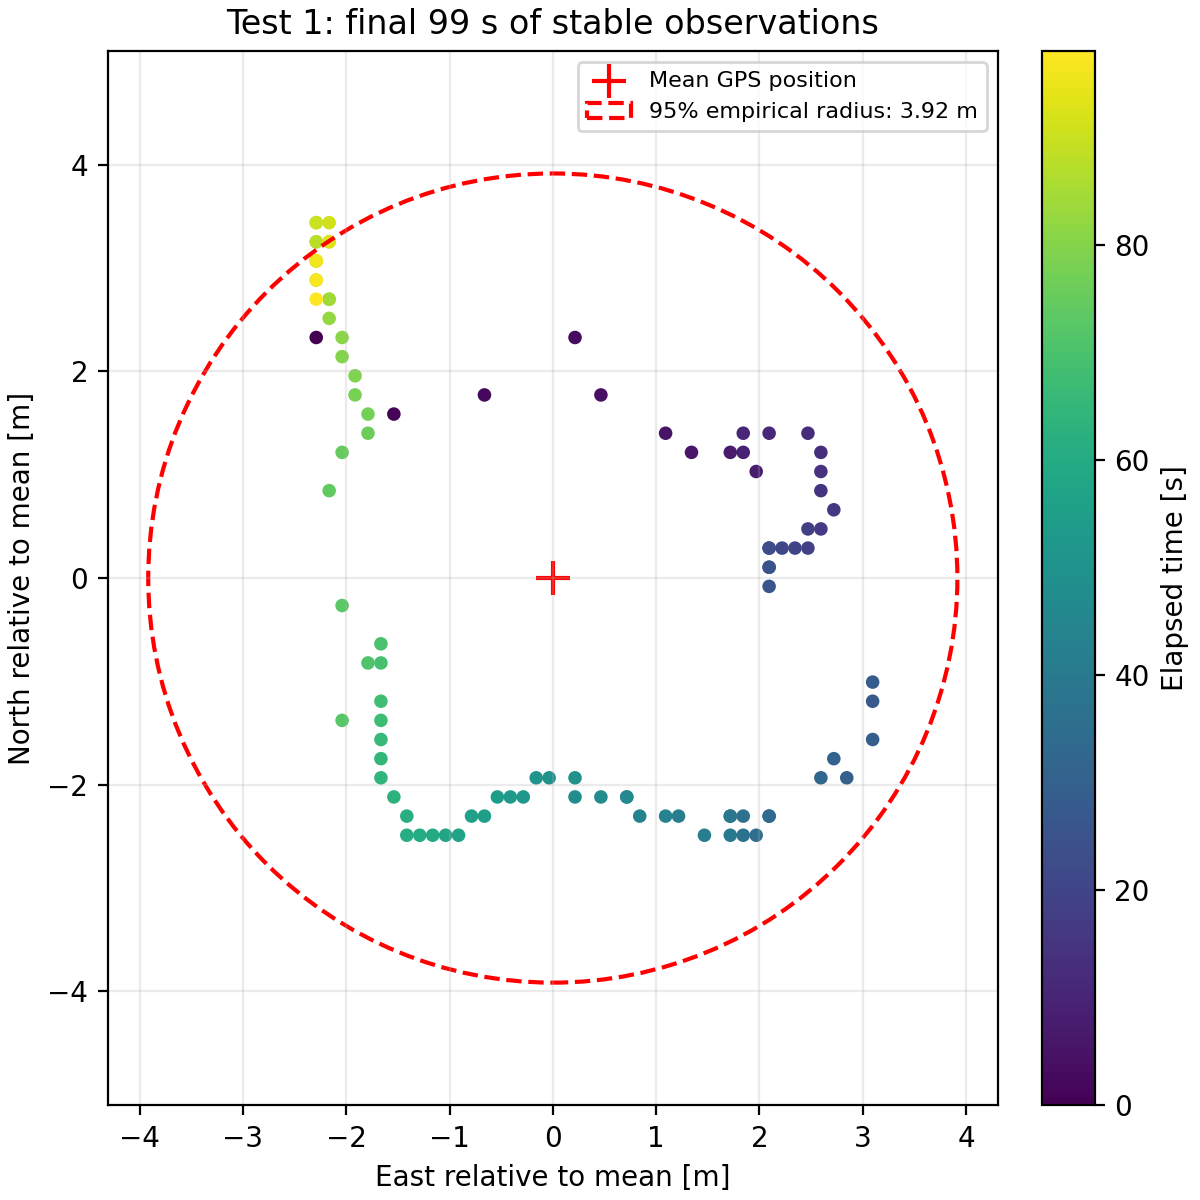
\includegraphics[width=0.61\textwidth]{stationary_scatter.png}
\caption{Stationary GPS measurements in the final 99 seconds, relative to their mean; the dashed circle has a radius of R95 = 3.92 m.}
\end{figure}

The large R95 for the complete stationary log is partly associated with GPS acquisition and weaker early geometry. In Test 1, the receiver initially reports 12 invalid position epochs; later it sometimes uses only three satellites, and the reported HDOP exceeds 50 during several intervals. For the final stable interval, the observed horizontal R95 of \textbf{approximately 4 m} is a reasonable empirical precision estimate. The overall R95 of \textbf{12.4 m} should also be reported rather than silently discarded. Neither result measures absolute GPS accuracy without a known true coordinate.

\section{Q3: Additional information from NMEA}

\begin{table}[H]
\centering
\small
\caption{Useful information available from the supplied NMEA sentence types.}
\begin{tabularx}{\textwidth}{@{}lX@{}}
\toprule
Message & Information available \\
\midrule
\texttt{RMC} & UTC date and time; data validity; latitude and longitude; speed over ground (knots); true course over ground. \\
\texttt{GGA} & Fix quality; number of satellites used; HDOP; altitude above mean sea level; geoid separation. \\
\texttt{GSA} & Automatic/manual mode; 2D or 3D position solution; satellite identifiers; PDOP, HDOP and VDOP. \\
\texttt{GSV} & Satellites in view; satellite identifiers; elevation, azimuth and signal strength when reported. \\
\texttt{VTG} & Ground-track angle and ground speed, reported in knots and km/h. \\
\bottomrule
\end{tabularx}
\end{table}

\clearpage
\subsection{Additional observations from these recordings}

\begin{itemize}
  \item \textbf{Date and timing:} The \texttt{RMC} field \texttt{041125} means 4 November 2025. Test 1 has 231 RMC epochs from 09:05:50 to 09:09:40 UTC, and Test 2 has 327 from 09:11:41 to 09:17:07 UTC.
  \item \textbf{Satellite availability:} Test 1 reports 5--10 satellites in view and uses 3--5 in its solution; Test 2 reports 13--14 in view and uses 6--7. Test 2 therefore has more satellites contributing to the position estimate.
  \item \textbf{Fix type and quality:} Of Test 1's accepted fixes, 77 have a 2D GSA solution and 142 a 3D solution. All 327 Test 2 fixes are 3D. Accepted GGA records have quality indicator 1 (standard GPS fix, not an RTK/differential fix).
  \item \textbf{Altitude and geoid:} GGA reports 106.6--108.9 m for Test 1 and 85.4--111.1 m for Test 2, with a geoid separation of 41.1 m. The approximately 26 m altitude range in Test 2 does not establish a true climb of that magnitude: GPS height is noisier than horizontal position.
  \item \textbf{Signal and satellite geometry:} The GSV fields describe satellite signal strength and sky positions; the GSA/GGA DOP values describe geometry (smaller generally indicates better geometry). Course angles at near-zero speed are unreliable as a heading estimate.
\end{itemize}

\section{Quality checks, limitations and conclusion}

The parser validated \textbf{all 1,040 NMEA sentences} in Test 1 and \textbf{all 1,568} in Test 2; no checksum failures were found. The first 12 invalid Test 1 epochs were excluded from position calculations. One valid RMC position is recorded approximately every second once a fix is available.

The combined evidence from speed and path shape shows that \textbf{Test 1 is stationary and Test 2 is moving}. Test 2 represents a short slow journey with changes of direction and a return close to the starting area. In stationary Test 1, the full-record empirical horizontal R95 is 12.39 m, while the final, more stable 99-second interval yields 3.92 m. These figures represent relative repeatability only. Satellite error, multipath, possible subtle physical motion, and time-correlated measurements can affect the estimates; HDOP cannot be directly converted into a meter error without a calibrated model.

\section*{References}
\begingroup
\small
\begin{enumerate}[leftmargin=*,label={[\arabic*]},itemsep=2pt]
 \item Garmin, \emph{NMEA 0183 sentence information}. \url{https://www8.garmin.com/manuals/webhelp/GUID-3E67C80C-0812-4EEC-BC60-699751B9CF6F/EN-US/GUID-891D6EC7-169E-4146-8279-8400626217D0.html}
 \item Trimble, \emph{NMEA-0183 GGA message reference}. \url{https://help.fieldsystems.trimble.com/r10/nmea0183-messages-gga.htm}
 \item Course assignment, \emph{GPS decoding and analysis}; supplied \texttt{nmea-test1-1.txt} and \texttt{nmea-test2-1.txt} recordings.
\end{enumerate}
\endgroup

\end{document}
